\chapter{Context}
\label{chap:context}
To motivate the quest for silicon sensors for experiments at high luminosity collider it is necessary 
to present first the theoretical context for experimental particle physics. In this Chapter a short 
reminder of the Standard Model of particle physics will be presented, with a special focus on 
the Higgs mechanism for the quarks, which is responsible for the mixing of quarks and the 
violation of the \CP symmetry in that sector.

\section{Introduction}
\label{sec:intro}

The Standard Model (SM) of particle physics~\cite{GLASHOW1961579,PhysRevLett.19.1264,SalamSM,PhysRevLett.30.1343,PhysRevLett.30.1346} is the theory describing three of the four known fundamental forces in the universe (the electromagnetic, weak, and strong interactions), as well as classifying all known elementary particles in leptons, quarks, gauge and scalar bosons. In Figure~\ref{fig:SM} a schematic summary of the SM 
particles.


\begin{figure}[htbp]
   \centering
   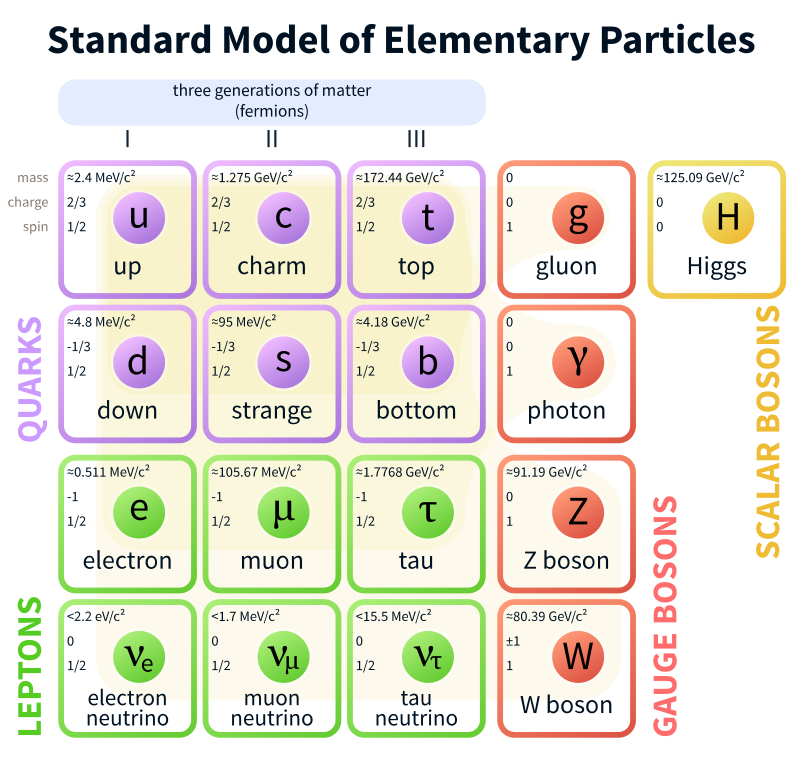
\includegraphics[width=0.5\textwidth]{SM.png} % requires the graphicx package
   \caption{The Standard Model of elementary particles, with the three generations of matter, gauge bosons in the fourth column, and the Higgs boson in the fifth~\cite{wiki:xxx}.}
   \label{fig:SM}
\end{figure}

The last member that was added to the set of SM particles was the so called Higgs boson, proposed in the '60s of the last century~(see for example~\cite{HIGGS1964132,PhysRevLett.13.321}),  finally observed in 2012~by the ATLAS and CMS collaborations~\cite{20121,201230}.
All massive SM particles acquire their rest mass by the interaction with the Higgs field, with different 
mechanisms for quarks and leptons (or ``fermions'') and for bosons. The details of the mechanism for 
the quarks will be presented in the next section.

\section{Mass terms in Standard Model Lagrangian and Quarks Mixing}
\label{sec:MassTermsSML}
As anticipated in the previous Section, in SM the elementary particles gain their mass through 
the so-called Higgs mechanism.
Adding a scalar field with a vacuum expectation value  $v$, the Lagrangian 
has appropriate mass terms.
The simplest model uses a Higgs doublet scalar field:

\begin{equation}
\phi=\left( \begin{array}{c}
\phi^{+} \\
\phi^{0}
\end{array} \right)
\label{eq:HiggsDoublet}
\end{equation}
where $\phi^{0,+}$ are complex fields.

The Yukawa couplings of fermions to Higgs field in the SM
 Lagrangian are given by:

\begin{equation}
\mathcal{L}_Y = - \sum_{i,j}\big(g^{ij}_d\overline Q_L^{i}\phi d_R^{j}
+ g^{ij}_u \overline Q_L^{i}\overline\phi u_R^{j} 
+ g^{ij}_{\ell} \overline L_L^{i}\phi\ell^j_R\big)+\rm{h.c.} 
\label{eq:YukLag}
\end{equation}
where $Q(L)$ represents the left handed quarks (leptons) doublets, the
 indices {\it i,j} run over the generations of fermions and
 $\overline \phi$ is the SU(2) doublet conjugate of $\phi$.
Couplings $g_u,\;g_d$ and $g_{\ell}$ are in general represented by
 complex matrices.

Inserting the expectation value $v$ in the Yukawa
 Lagrangian~\ref{eq:YukLag}, we obtain:

\begin{equation}
\mathcal{L}_{\rm{Y}} = - \sum_{k=u,d,\ell} \overline k_L\mathcal{M}_k k_R
\label{eq:YukLagExp}
\end{equation}
where $\mathcal{M}_k^{ij} = vg_k^{ij}$ are mass matrices. In general these 
matrices are not diagonal and  therefore introduce mixing between the
 different generations of quarks. Hence, the
 SM Lagrangian is not expressed in terms of mass eigenstates but instead
in terms of the eigenstates of the weak interactions.
   We can, however, rewrite the fields using a unitary transformation:

\begin{equation}
\begin{array}{ccc}
u_l = V^u_L u'_L & , & u_R = V^u_R u'_R \\
d_l = V^d_L d'_L & , & d_R = V^d_R d'_R \\
\label{eq:MatrRot}
\end{array}
\end{equation}
so $\mathcal{M}'=V^{\dagger k}_L\mathcal{M}_kV_R^k$ is the diagonal mass
 matrix.





Quark mass eigenstates are different from weak interaction
 eigenstates; we may want to write weak interactions in the mass
 eigenstate base.

Charged current weak interactions can be described in SM by the product of
 an operator $J^{\mu}$ (with $V-A$ structure) and the \W boson:

\begin{equation}
\mathcal{L}_{int}=-\frac{g}{\sqrt{2}}(\mathcal{J^{\mu}}\W_{\mu}^{+}+\mathcal{J^{\mu\dagger}}\W_{\mu}^{-})
\label{eq:LintWeak}
\end{equation}
where $g$ is the weak charge related to Fermi coupling constant by 
$G_F/\sqrt{2}=g^2/8M_W^2$, where $M_W$ is the \W boson mass.

Weak charged current for quarks are written then in this way:

\begin{equation}
\mathcal{J}^{\mu} = \sum_{i,j} V_{ij}J^{\mu}_{ij} = 
\sum_{i,j}\ubar_i' \gamma^{\mu}\frac{1}{2}(1-\gamma_5)V^{CKM}_{ij}d_j'
\label{eq:ChCurr}
\end{equation}
where $V^{CKM}_{ij}$ are the terms of Cabibbo, Kobayashi and Maskawa (CKM) 
matrix~\cite{PhysRevLett.10.531,Kobayashi:1973fv}, which is defined as $V_L^{\dagger u}V_L^{d}$ 
(see eq.~\ref{eq:MatrRot}), and is usually written in this form:

\begin{equation}
V=
\left( \begin{array}{ccc}
V_{ud} & V_{us} & V_{ub} \\
V_{cd} & V_{cs} & V_{cb} \\
V_{td} & V_{ts} & V_{tb}
\end{array} \right)
\label{eq:CKM}
\end{equation}


Quark mixing idea was first introduced by Cabibbo~\cite{PhysRevLett.10.531} in 1963 
to explain weak transition among different quark generations. 
Christensen {\it et al.}~\cite{PhysRevLett.13.138} observed \CP violation in
 neutral kaon system in 1964 
 Kobayashi and Maskawa~\cite{Kobayashi:1973fv} in 1973 proposed a third quark family and a
 complex phase in quark mixing matrix to accommodate \CP violation in
 Standard Model.

Quark mixing matrix parameters are unbounded from theory and need to be 
experimentally determined. 

\section{Tracking and Vertexing for Experimental Particle Physics}

All the theoretical predictions about elementary particles presented in the previous sections 
(and many more) 
have been validated thanks to decades of experiments. In experimental particle physics we 
want to 
reconstruct the tracks and energy deposits of particles produced in collisions and measure their 
characteristics, like: energy, momentum, charge, and their lifetime, if it applies.
If we now restrict to charged particles we can measure their production and decay vertex thanks to 
the reconstruction of their trajectory; the distance between these two vertices is proportional to the 
lifetime of the particle (see also Figure~\ref{fig:HFDV}).

\begin{figure}[htbp]
   \centering
   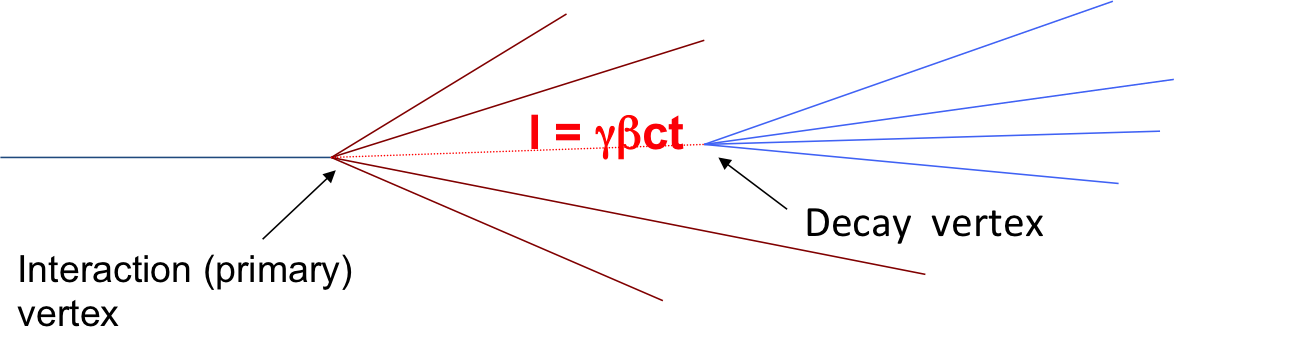
\includegraphics[width=0.66\textwidth]{lifetime.png} % requires the graphicx package
   \caption{Schematic view of production and decay vertex of heavy flavour particles.}
   \label{fig:HFDV}
\end{figure}

Lifetimes of $\tau$ leptons, charm 
and beauty hadrons range from 0.2 to 1.5~ps; these ranges of lifetimes means that these particles 
fly distances of single millimetres from the interaction vertex inside modern high energy physics 
experiments\footnote{This characteristic is also exploited to ``tag'' the flavour of particles, like $b$ and 
$c$ quarks. This will be discussed in more detail in Chapter~\ref{chap:ATLAS}}. To achieve the measurement goals we set above we then need particle detectors
with sub-millimeter precision.

Another example of the spatial precision required by particle physics comes from the 
so called ``B Factories''. At the Stanford Linear Accelerator Center (SLAC) 
asymmetric-energy electron-positron collider PEP-II~\cite{37821} the \Y4S resonance was produced 
with a net boost in the laboratory frame. This configuration allowed to separate the subsequent 
decay vertices of the two \B mesons produced by the \Y4S decay. In Figure~\ref{fig:BFCPV} 
a schematic view of the working principle of the B Factories. 

\begin{figure}[htbp]
   \centering
   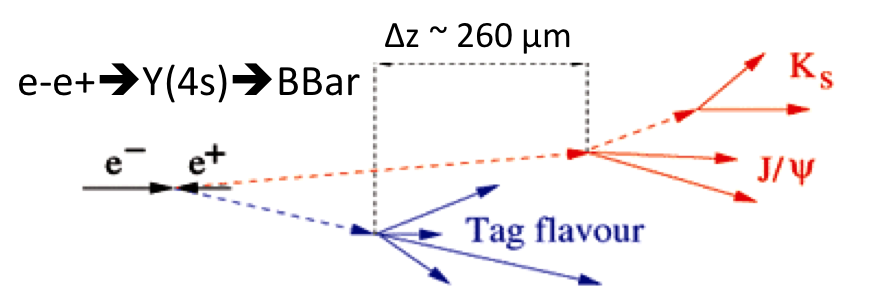
\includegraphics[width=0.66\textwidth]{BFCPV.png} % requires the graphicx package
   \caption{Schematic view of the B Factories working principle.}
   \label{fig:BFCPV}
\end{figure}

Thanks to the Lorentz boost $\beta\gamma$ of about 0.56 the decay vertices of the two \B mesons 
could be separated by about 260~$\mum$ along the beam axis. Hence, to precisely measure these 
two vertices a detector with a spatial resolution of the order of $260/3\sim80$~$\mum$ was needed.
The \babar~detector~\cite{AUBERT20021} recorded the events produced at the PEP-II collider; 
at the core of the \babar~detector there was the \babar~Silicon Vertex Tracker~(SVT),  the most relevant detector for the measurement of time dependent \CP asymmetries in \babar. The \babar~SVT 
was composed of five roughly cylindrical detection layers, made of double sided silicon strip modules. 
In order not to degrade by more than 10\% the precision of  \CP violation measurements, the resolution 
was required to be better than 80~$\mum$ on fully reconstructed \B decay vertices.

\section{Space Point and Secondary Vertex Measurements}
\label{sec:SPmeas}

We now analyse the achievable precision on momentum resolution and on secondary vertex 
reconstruction; the goal is to understand their dependence on the geometry of the tracker, on its 
material budget and its measurement precision. 

The base of tracking and vertexing is the measurement of space-points, {\it i.e.} the 3D position 
of the track traversing the sensing layer. This is the result of electrons and holes, produced by the 
track passing through the sensor bulk, collected by the sensing electrodes and digitised by the 
readout electronics. Diffusion and Lorentz angle deviation 
can deteriorate the space-point measurement precision; more details in Chapter~\ref{chap:silicon}.

Assuming a space point-resolution of $\sigma_{point}$, the (transverse) momentum resolution is~\cite{GLUCKSTERN1963381,Olive:2016xmw,Garcia-Sciveres:2017ymt}:

\begin{equation}
\dfrac{\sigma_{p_{T}}}{p_{T}} = \Bigg( \dfrac{p_T}{0.3|z|}\dfrac{\sigma_{point}}{L^2B}\sqrt{\dfrac{720}{N+4}}\Bigg) \oplus \Bigg(\dfrac{\sigma_{p_{T}}}{p_{T}}\Bigg)_{MS}
\label{eq:ptres}
\end{equation} 

where $p_T$ is the particle momentum (in GeV/c) transverse to the magnetic field $B$ (in Tesla); 
$L$ is the the radial length, in meters (the space point-resolution of $\sigma_{point}$ is measured in 
meters too). $N$ is the numbers of measuring layers in the tracker and for this formulation it is 
assumed to be large. As it can be seen from Equation~\ref{eq:ptres}, other than a good 
space-point resolution, it is also important to have a large magnetic field and a long tracker lever 
arm; the latter in particular enters quadratically in the formula. 

The charged particles ionise the medium through Coulomb interactions, which involve energy and 
{\it momentum} exchanges, hence the particle being tracked is subject to many (small) deflections. 
The collective name for all these deflections is {\it multiple scattering} (MS). MS deteriorates the 
momentum resolution by ~\cite{Garcia-Sciveres:2017ymt}:

\begin{equation}
\Bigg(\dfrac{\sigma_{p_{T}}}{p_{T}}\Bigg)_{MS} = \dfrac{0.054}{\beta B L/\sin\theta}\sqrt{\dfrac{x/\sin\theta}{X_0}}
\label{eq:MS}
\end{equation} 
with $L$ and $B$ as in Equation~\ref{eq:ptres}. Here $L/\sin\theta$ is the projected tracker length
 and $(x/\sin\theta)/X_0$ is the material thickness traversed by the particle, expressed in unit 
 of radiation length $X_0$, when the particle crosses the detector at an angle $\theta$ with respect 
 to the detector surface.
 
 As an example, the resolution of a 1~GeV/c $p_T$ track in a $L=1$~m 
 $N=10$ layers 
 tracker, immersed in a $B=$1~T solenoidal field, is about 1.0\% if the space-point resolution   
 $\sigma_{point}$ is about 10~$\mu$m for tacks at normal incidence; the result is dominated by 
 MS effect. For a 100~GeV/c $p_T$ the resolution is about 2.0\% and it is dominated by the 
 error on the curvature measurement (first term of Equation~\ref{eq:ptres}).

The error on secondary vertex reconstruction is linked to the precision on 
transverse impact parameter $d_0$~\cite{Garcia-Sciveres:2017ymt}:

\begin{equation}
\sigma_{d0}\approx\dfrac{\sigma_{point}}{\sqrt{N}}\sqrt{1+\dfrac{12(N-1)}{N+1}\Big(\dfrac{r}{L}\Big)^2}\oplus\theta_0 r_{pv}\sqrt{\dfrac{N(2N-1)}{6(N-1)^2}}
\label{eq:d0res}
\end{equation} 
where the first term results from the extrapolation from the tracker to the primary vertex with $r/L$
being the ratio of the extrapolation distance to the tracker length. It is clear it is better to have 
the first layer as close as possible to the interaction point (small $r$), and then have 
subsequent layers as far as possible (large $L$); increasing the number $N$ of measurements 
help as usual (central limit theorem); the resolution depends 
linearly on the space-point resolution. The second term is due to multiple scattering, where 
$\theta_0$ is the the multiple scattering angle~\cite{Olive:2016xmw}, and and $r_{pv}$ the distance 
of the first  layer to the primary interaction vertex. Minimising material and getting layer as 
close as possible to the primary vertex helps; on the contrary, adding many layers here don't work 
since each layer adds to the material budget, hence makes the MS effect more and more important.

For a 4-layer geometry like in ATLAS (see Figure~\ref{fig:ATLASID}) and a material thickness of 
typically around  3\% $X_0$ this yields~\cite{Garcia-Sciveres:2017ymt}:

\begin{equation}
\sigma_{d_{0}}=\dfrac{90\,\mu {\rm m\,GeV/c}}{p}
\end{equation}

\section{Summary}
The few examples above show the importance of sub-millimeter precision in determining elementary 
particles production  and decay vertices, not only to measure  particles' lifetimes but also 
to make fundamental measurements possible, like assessing the  \CP violation in the \B meson 
sector. We will see in the next Chapter why silicon detectors are the standard choice for tracking and 
vertexing in High Energy physics experiments.
